\documentclass[aspectratio=43]{beamer}

% Title --------------------------------------------
\title{\huge Civil wars II}
\author{Francisco Villamil}
\date{War, peace, and political violence\\UC3M, Fall 2023}

%%% NOTE -- CHECK THIS: https://github.com/paulgp/beamer-tips


%%% Building heavily on https://github.com/kylebutts/templates

% xcolor, define them
\usepackage{xcolor}

% TEXT COLORS
\definecolor{red}{HTML}{9a2515}
\definecolor{yellow}{HTML}{EBC944}
\definecolor{asher}{HTML}{555F61}
\definecolor{jet}{HTML}{131516}

% THEME COLORS
\definecolor{accent}{HTML}{107895}
\definecolor{accent2}{HTML}{9a2515}

% Color commands
\newcommand\red[1]{{\color{red}#1}}
\newcommand\yellow[1]{{\color{yellow}#1}}
\newcommand\asher[1]{{\color{asher}#1}}

\newcommand\BGred[1]{{\colorbox{red!80!white}{#1}}}
\newcommand\BGyellow[1]{{\colorbox{yellow!80!white}{#1}}}
\newcommand\BGasher[1]{{\colorbox{asher!80!white}{#1}}}

\renewcommand<>{\BGyellow}[1]{\only#2{\beameroriginal{\BGyellow}}{#1}}

% Appendix numbering
\usepackage{appendixnumberbeamer}

% Beamer Options -------------------------------------

% Background
\setbeamercolor{background canvas}{bg = white}

% Change text margins
\setbeamersize{text margin left = 25pt, text margin right = 15pt}

% \alert
\setbeamercolor{alerted text}{fg = accent2}

% Frame title
\setbeamercolor{frametitle}{bg = white, fg = jet}
\setbeamercolor{framesubtitle}{bg = white, fg = accent}
\setbeamerfont{framesubtitle}{size = \small, shape = \itshape}

% Block
\setbeamercolor{block title}{fg = white, bg = accent2}
\setbeamercolor{block body}{fg = jet, bg = jet!10!white}

% Title page
\setbeamercolor{title}{fg = jet}
\setbeamercolor{subtitle}{fg = accent}

%% Custom \maketitle and \titlepage
\setbeamertemplate{title page}
{
    \begin{centering}
      % \vspace{20mm}
      {\Large \usebeamerfont{title}\usebeamercolor[fg]{title}\inserttitle}\\ \vskip0.25em%
      \ifx\insertsubtitle\@empty%
      \else%
        {\usebeamerfont{subtitle}\usebeamercolor[fg]{subtitle}\insertsubtitle\par}%
      \fi%
      {\vspace{10mm}\insertauthor}\\
      \ifx\insertinstitute\@empty%
      \else%
        {\vspace{5mm}\color{asher}\scriptsize{\insertinstitute}}
      \fi%
      {\color{asher}\small{\insertdate}}\\
    \end{centering}
}

% Table of Contents
\setbeamercolor{section in toc}{fg = accent!70!jet}
\setbeamercolor{subsection in toc}{fg = jet}

% Button
\setbeamercolor{button}{bg = accent}

% Remove navigation symbols
\setbeamertemplate{navigation symbols}{}

% Table and Figure captions
\setbeamercolor{caption}{fg=jet!70!white}
\setbeamercolor{caption name}{fg=jet}
\setbeamerfont{caption name}{shape = \itshape}

% Put slide number / total slides at the bottom right
\makeatother
\makeatletter
\setbeamertemplate{footline} %{\hfill\insertframenumber/\inserttotalframenumber}
{%
  \leavevmode%
  \hbox{
  \begin{beamercolorbox}[wd=\paperwidth,ht=2.5ex,dp=1.125ex,leftskip=.3cm,rightskip=.3cm plus1fil]{footlinecolor}%
    \color{asher}{\hfill\insertframenumber/\inserttotalframenumber}
  \end{beamercolorbox}}%
  \vskip0pt%
}
\makeatother
\makeatletter

% Bullet points

%% Fix left-margins
\settowidth{\leftmargini}{\usebeamertemplate{itemize item}}
\addtolength{\leftmargini}{\labelsep}

%% enumerate item color
\setbeamercolor{enumerate item}{fg = accent}
\setbeamerfont{enumerate item}{size = \small}
\setbeamertemplate{enumerate item}{\insertenumlabel.}

%% itemize
\setbeamercolor{itemize item}{fg = accent!70!white}
\setbeamerfont{itemize item}{size = \small}
\setbeamertemplate{itemize item}[circle]
\setlength{\itemsep}{0pt plus 6pt}

%% right arrow for subitems
\setbeamercolor{itemize subitem}{fg = accent!60!white}
\setbeamerfont{itemize subitem}{size = \small}
\setbeamertemplate{itemize subitem}{$\rightarrow$}

\setbeamertemplate{itemize subsubitem}[square]
\setbeamercolor{itemize subsubitem}{fg = jet}
\setbeamerfont{itemize subsubitem}{size = \small}

% References

%% Bibliography Font, roughly matching aea
\setbeamerfont{bibliography item}{size = \footnotesize}
\setbeamerfont{bibliography entry author}{size = \footnotesize, series = \bfseries}
\setbeamerfont{bibliography entry title}{size = \footnotesize}
\setbeamerfont{bibliography entry location}{size = \footnotesize, shape = \itshape}
\setbeamerfont{bibliography entry note}{size = \footnotesize}

\setbeamercolor{bibliography item}{fg = jet}
\setbeamercolor{bibliography entry author}{fg = accent!60!jet}
\setbeamercolor{bibliography entry title}{fg = jet}
\setbeamercolor{bibliography entry location}{fg = jet}
\setbeamercolor{bibliography entry note}{fg = jet}

%% Remove bibliography symbol in slides
\setbeamertemplate{bibliography item}{}





% Links ----------------------------------------------

\usepackage{hyperref}
\hypersetup{
  colorlinks = true,
  linkcolor = accent,
  filecolor = accent,
  urlcolor = accent,
  citecolor = accent,
}


% Line spacing --------------------------------------
\usepackage{setspace}
\setstretch{1.2}


% \begin{columns} -----------------------------------
\usepackage{multicol}


% % Fonts ---------------------------------------------
% % Beamer Option to use custom fonts
% \usefonttheme{professionalfonts}
%
% % \usepackage[utopia, smallerops, varg]{newtxmath}
% % \usepackage{utopia}
% \usepackage[sfdefault,light]{roboto}
%
% % Small adjustments to text kerning
% \usepackage{microtype}



% Remove annoying over-full box warnings -----------
\vfuzz2pt
\hfuzz2pt


% Table of Contents with Sections
\setbeamerfont{myTOC}{series=\bfseries, size=\Large}
\AtBeginSection[]{
        \frame{
            \frametitle{Roadmap}
            \tableofcontents[current]
        }
    }


% References ----------------------------------------
\usepackage[
    citestyle= authoryear,
    style = authoryear,
    natbib = true,
    backend = biber
]{biblatex}

% Smaller font-size for references
\renewcommand*{\bibfont}{\small}

% Remove "In:"
\renewbibmacro{in:}{}

% Color citations for slides
\newenvironment{citecolor}
    {\footnotesize\begin{color}{accent2}}
    {\end{color}}

\newcommand{\citetcolor}[1]{{\footnotesize\textcolor{asher}{\citet{#1}}}}
\newcommand{\citepcolor}[1]{{\footnotesize\textcolor{asher}{\citep{#1}}}}

% Tables -------------------------------------------
% Tables too big
% \begin{adjustbox}{width = 1.2\textwidth, center}
\usepackage{adjustbox}
\usepackage{array}
\usepackage{threeparttable, booktabs, adjustbox}

% Fix \input with tables
% \input fails when \\ is at end of external .tex file

\makeatletter
\let\input\@@input
\makeatother

% Tables too narrow
% \begin{tabularx}{\linewidth}{cols}
% col-types: X - center, L - left, R -right
% Relative scale: >{\hsize=.8\hsize}X/L/R
\usepackage{tabularx}
\newcolumntype{L}{>{\raggedright\arraybackslash}X}
\newcolumntype{R}{>{\raggedleft\arraybackslash}X}
\newcolumntype{C}{>{\centering\arraybackslash}X}

% Figures

% \imageframe{img_name} -----------------------------
% from https://github.com/mattjetwell/cousteau
\newcommand{\imageframe}[1]{%
    \begin{frame}[plain]
        \begin{tikzpicture}[remember picture, overlay]
            \node[at = (current page.center), xshift = 0cm] (cover) {%
                \includegraphics[keepaspectratio, width=\paperwidth, height=\paperheight]{#1}
            };
        \end{tikzpicture}
    \end{frame}%
}

% subfigures
\usepackage{subfigure}


% Highlight slide -----------------------------------
% \begin{transitionframe} Text \end{transitionframe}
% from paulgp's beamer tips
\newenvironment{transitionframe}{
    \setbeamercolor{background canvas}{bg=accent!60!black}
    \begin{frame}\color{accent!10!white}\LARGE\centering
}{
    \end{frame}
}


% Table Highlighting --------------------------------
% Create top-left and bottom-right markets in tabular cells with a unique matching id and these commands will outline those cells
\usepackage[beamer,customcolors]{hf-tikz}
\usetikzlibrary{calc}
\usetikzlibrary{fit,shapes.misc}

% To set the hypothesis highlighting boxes red.
\newcommand\marktopleft[1]{%
    \tikz[overlay,remember picture]
        \node (marker-#1-a) at (0,1.5ex) {};%
}
\newcommand\markbottomright[1]{%
    \tikz[overlay,remember picture]
        \node (marker-#1-b) at (0,0) {};%
    \tikz[accent!80!jet, ultra thick, overlay, remember picture, inner sep=4pt]
        \node[draw, rectangle, fit=(marker-#1-a.center) (marker-#1-b.center)] {};%
}



\begin{document}

\begin{frame}
  \titlepage
\end{frame}

% ----------------------------------------------------
\begin{frame}
\frametitle{Greed \& opportunity}
\centering

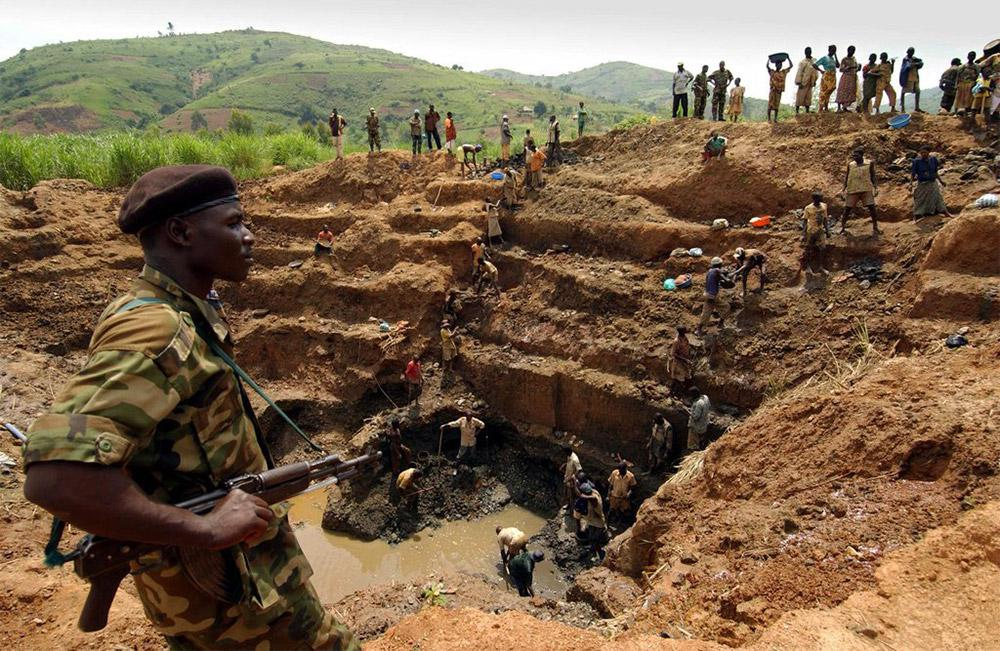
\includegraphics[width = 0.8\textwidth]{img/conflict_diamonds}

\vspace{10pt}
{\small Gold mine in Ituri region, eastern Democratic Republic of Congo (2003)}

\end{frame}
% ----------------------------------------------------

% ----------------------------------------------------
\begin{frame}
\frametitle{Greed \& opportunity}
\centering

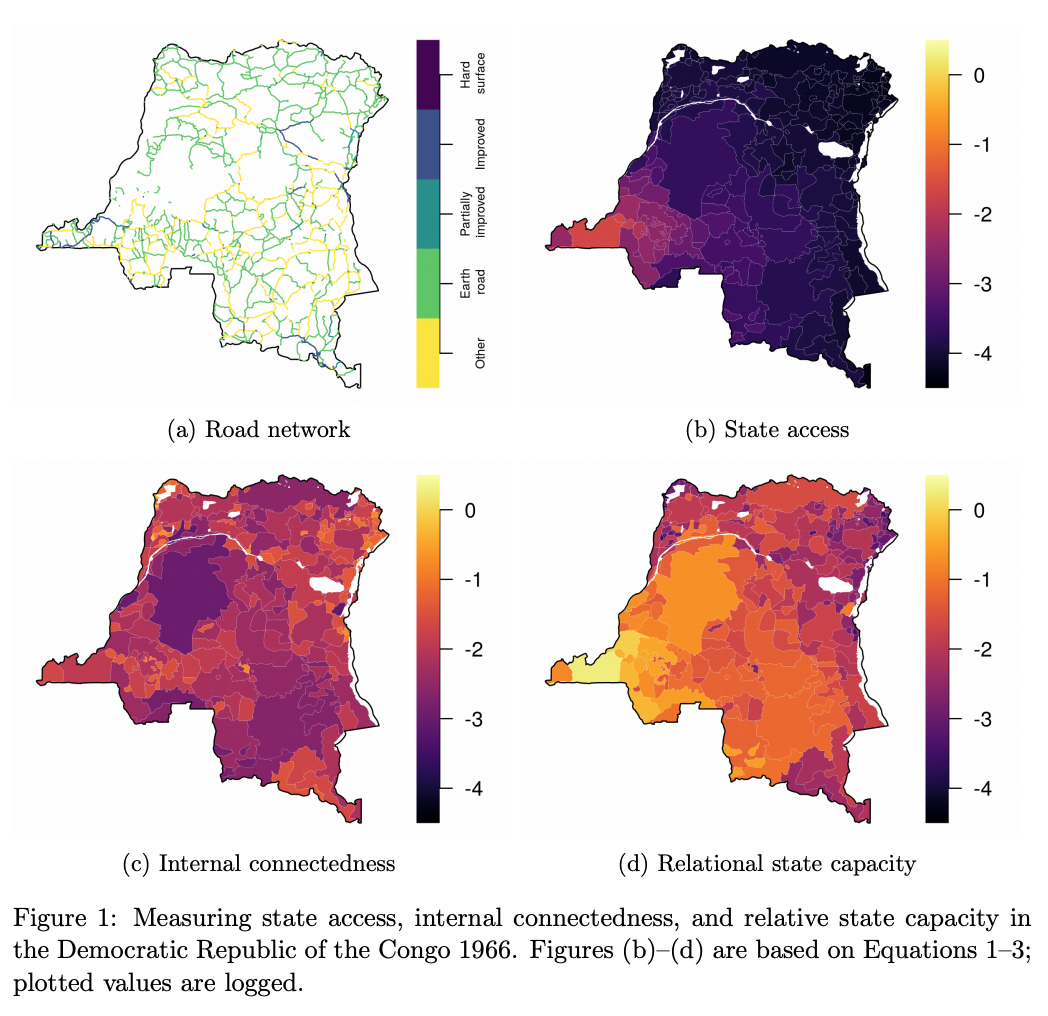
\includegraphics[width = 0.7\textwidth]{img/muller-crepon}

{\small (Müller-Crepon \textit{et al.}, 2020)}

\end{frame}
% ----------------------------------------------------

% ----------------------------------------------------
\begin{frame}
\frametitle{Greed \& opportunity: what they have in common}
\centering

\begin{itemize}
  \item Ruling out \textit{motivational} factors related to ideology, religion, ethnicity, inequality...
  \item Previous explanations based on grievances do not work
  \item Grievances are ubiquitous, so they can't explain anything
  \item Empirical results: no effect of ethnic fractionalization
  \begin{itemize}
    \item Ethnic fractionalization: probability that two randomly drawn individuals belong to the same ethnic group (more ethnic groups, higher fractionalization)
  \end{itemize}
\end{itemize}

\end{frame}
% ----------------------------------------------------

% ----------------------------------------------------
\begin{frame}
\frametitle{What are grievances?}
\centering

\includegraphics[width = 0.6\textwidth]{img/revolt1381}

% {\small (English 1381 Peasants' Revolt)}
\begin{itemize}
  \item Outrage and historical rebellions
\end{itemize}

\end{frame}
% ----------------------------------------------------

% ----------------------------------------------------
\begin{frame}
\frametitle{What are grievances?}
\centering

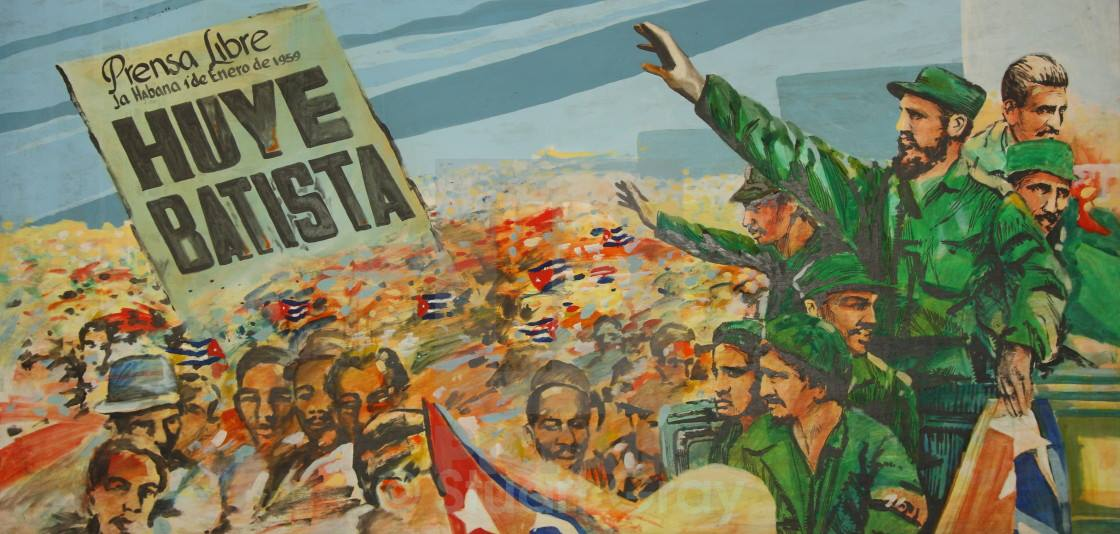
\includegraphics[width = \textwidth]{img/cuba}

\begin{itemize}
  \item Outrage and contemporary revolutions
\end{itemize}

\end{frame}
% ----------------------------------------------------

% ----------------------------------------------------
\begin{frame}
\frametitle{Grievances \& ideology in the greed perspective}
\centering

\begin{minipage}{0.55\textwidth}\centering
\begin{itemize}
  \item Rebels `wrap' themselves in ideology
  \item But no real effect: we won't be able to predict the outbreak of civil wars based on the existence of grievances
  \item Is this true?
\end{itemize}
\end{minipage}\hfill
\begin{minipage}{0.44\textwidth}\centering
  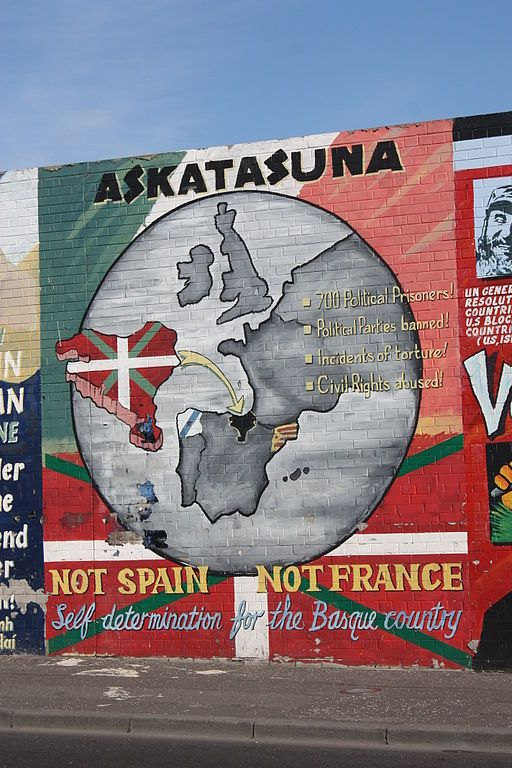
\includegraphics[width = 0.9\textwidth]{img/belfast_mural}

  {\small Mural in Belfast}
\end{minipage}

\end{frame}
% ----------------------------------------------------

% ----------------------------------------------------
\begin{frame}
\frametitle{The first wave of grievance studies}
\centering

\begin{minipage}{0.59\textwidth}\centering
\begin{itemize}
  \item Context in the 60s: violence and revolution in the `Third World,' civil rights movement in the US
  \item What brings men and women to rise against `unjust' regimes?
  \item Focus on psychological mechanisms
  \item `Relative deprivation:' frustration over unmet expectations of material wellbeing triggers violent behavior
  \begin{itemize}
    \item In other words: `I'm not getting what I deserve'
  \end{itemize}
\end{itemize}
\end{minipage}\hfill
\begin{minipage}{0.4\textwidth}\centering
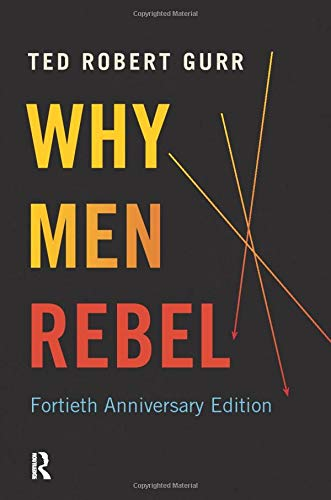
\includegraphics[width = 0.9\textwidth]{img/why_men_rebel}

Ted Gurr (1970)
\end{minipage}

\end{frame}
% ----------------------------------------------------

% ----------------------------------------------------
\begin{frame}
\frametitle{The first wave of grievance studies}
\centering

\begin{itemize}
  \item Different from previous sociological theories of mob behavior, irrational mass behavior, etc
  \item Influenced by the ideological conflict of the Cold War
  \item Civil wars interpreted as `peasant revolutions' or `social revolutions'
\end{itemize}

\end{frame}
% ----------------------------------------------------

% ----------------------------------------------------
\begin{frame}
\frametitle{The first wave of grievance studies}
\centering

\begin{minipage}{0.59\textwidth}\centering
\begin{itemize}
  \item Rebellions in Burma, Cochinchina
  \item Subsistence economy, social reciprocity
  \item Traditional (feudal) moral economy that preserved subsistence, social preference for stability
  \item Market-based transformations destroy this moral equilibrium and breed rebellion
\end{itemize}
\end{minipage}\hfill
\begin{minipage}{0.4\textwidth}\centering
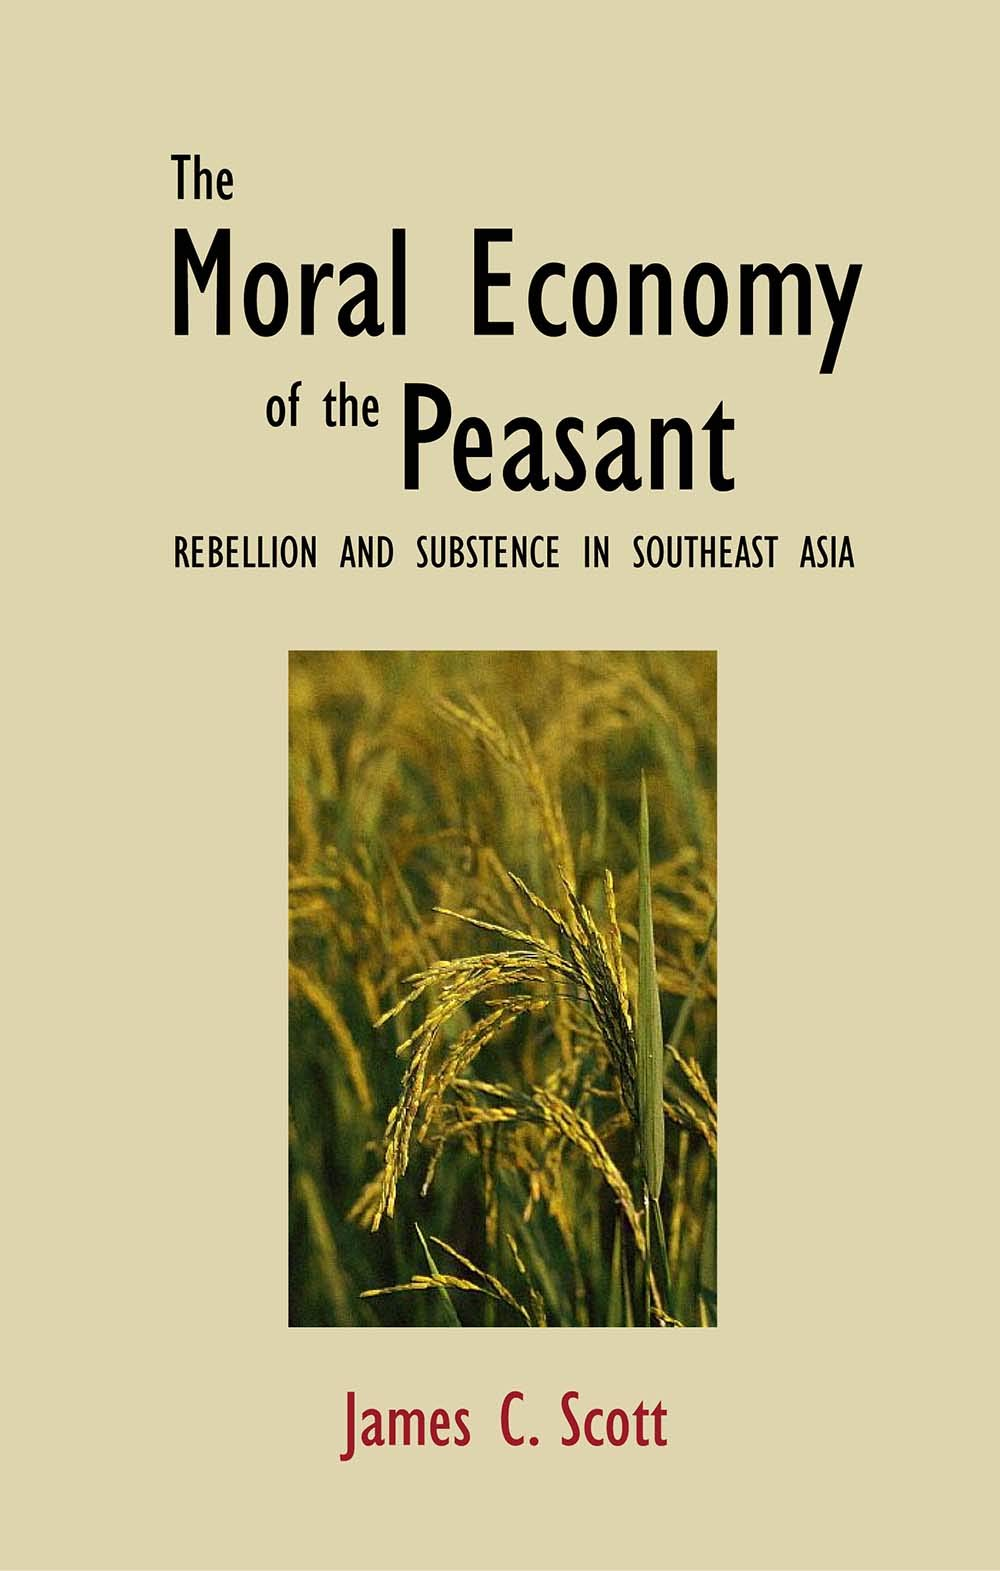
\includegraphics[width = 0.9\textwidth]{img/scott_moral}

James C Scott (1976)
\end{minipage}

\end{frame}
% ----------------------------------------------------

% ----------------------------------------------------
\begin{frame}
\frametitle{The first wave of grievance studies}
\centering

\begin{minipage}{0.59\textwidth}\centering
\begin{itemize}
  \item French, Russian, and Chinese Revolutions
  \item Social revolutions as a radical transformation of social and political structures (not a rebellion, not a political revolution)
  \item State-centric explanation of revolutions as a product of class struggle
\end{itemize}
\end{minipage}\hfill
\begin{minipage}{0.4\textwidth}\centering
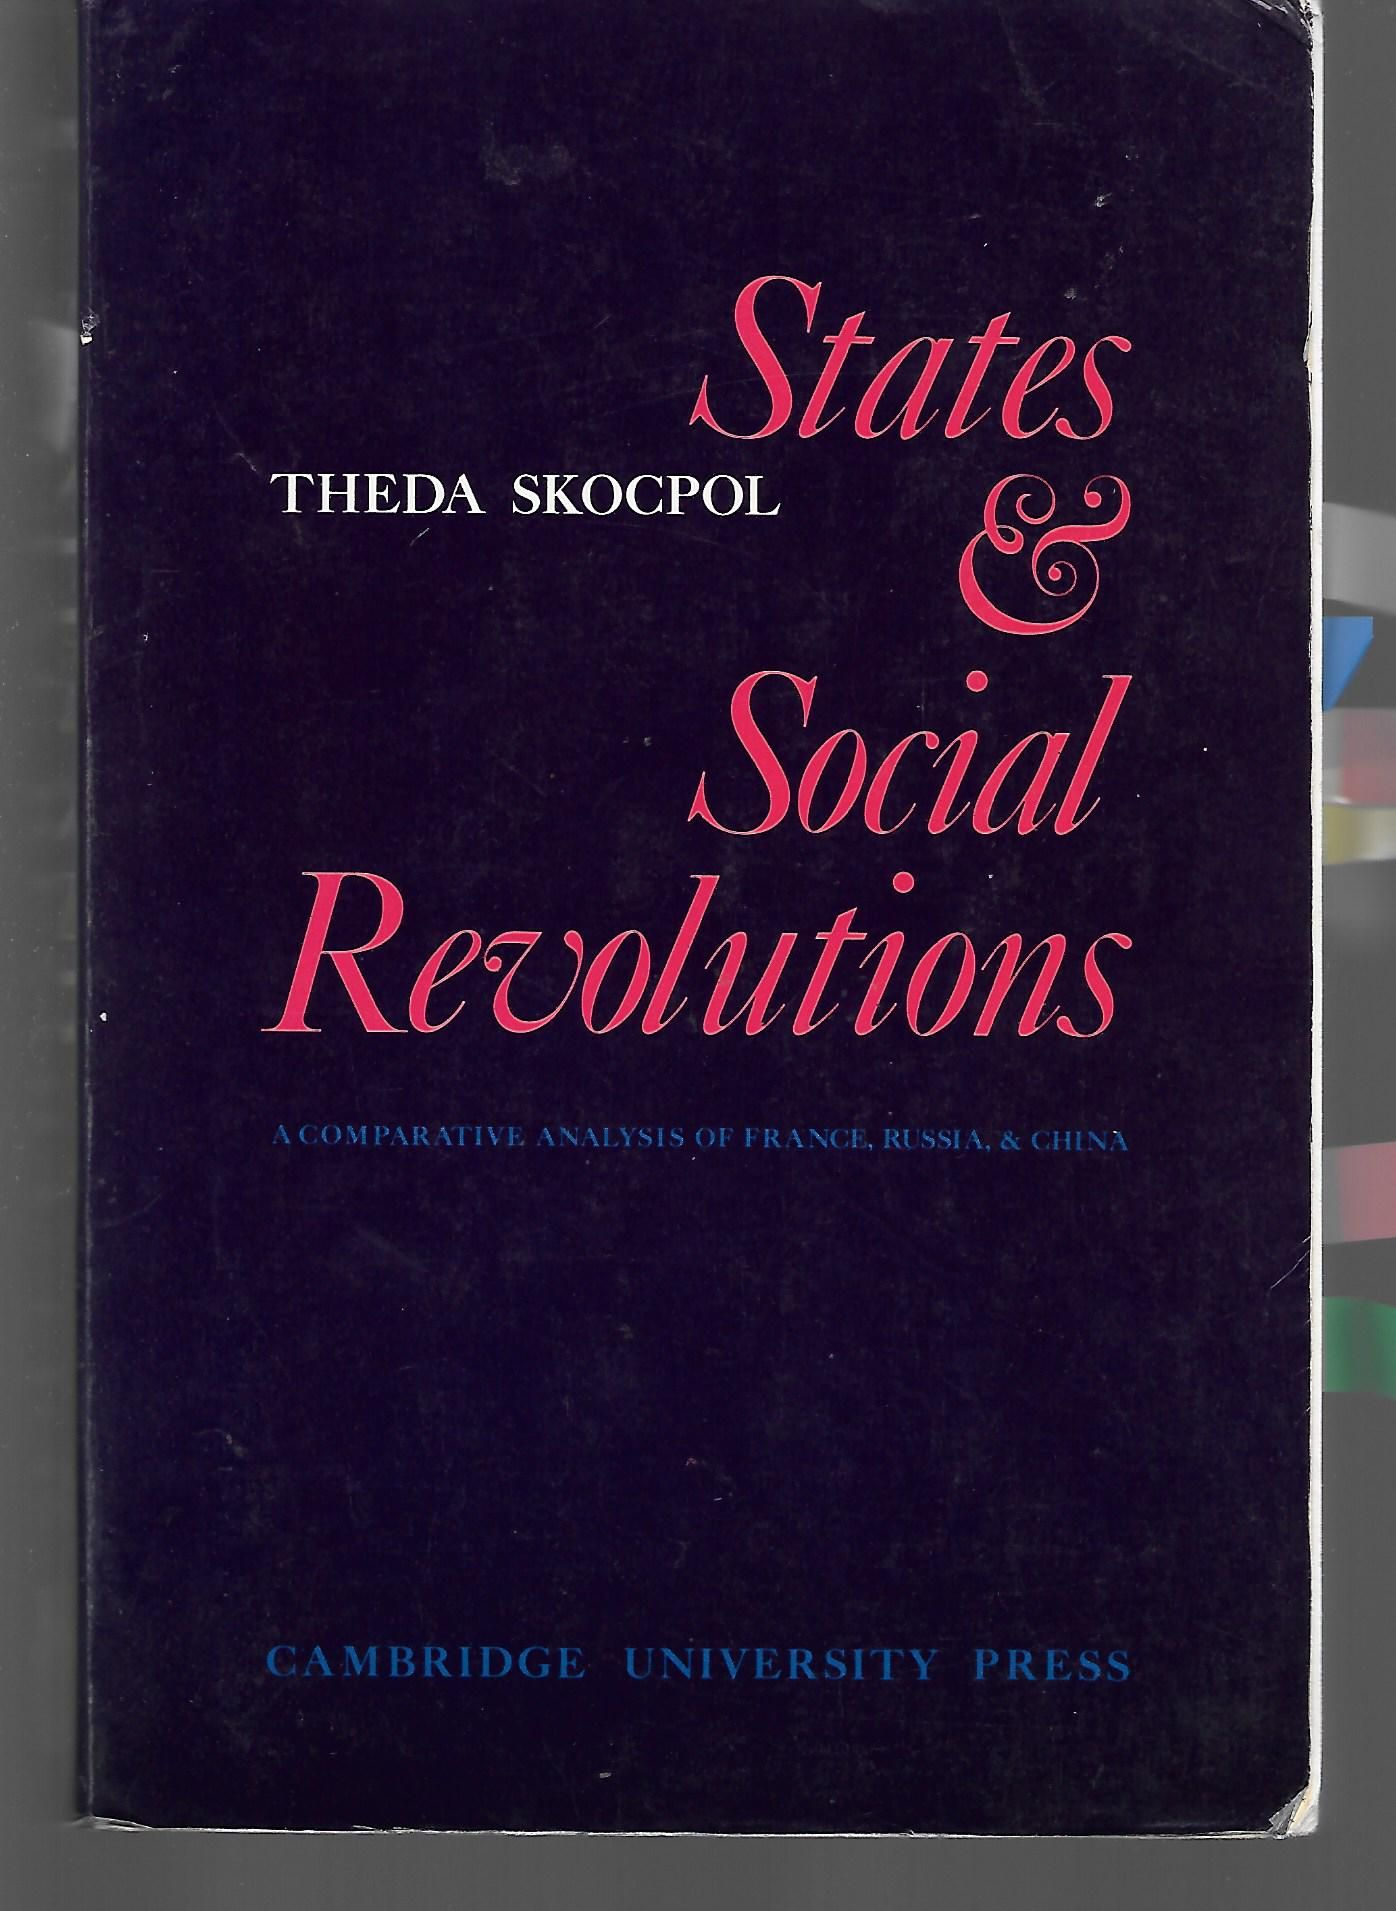
\includegraphics[width = 0.9\textwidth]{img/skocpol}

Theda Skocpol (1979)
\end{minipage}

\end{frame}
% ----------------------------------------------------

% ----------------------------------------------------
\begin{frame}
\frametitle{The first wave of grievance studies}
\centering

\begin{quote}
No social group is more conservative than a landowning peasantry and none is more revolutionary than a peasantry that owns too little land or pays too high a rental.
\end{quote}

\vspace{10pt}

{\footnotesize Samuel P Huntington (1968) \textit{Political Order in Changing Societies,} p. 375.}

\end{frame}
% ----------------------------------------------------

% ----------------------------------------------------
\begin{frame}
\frametitle{Early criticism or contributions}
\centering

\begin{itemize}
  \item Collective action theory and the focus on opportunity structures (Tilly, \textit{From Mobilization to Revolution}): individual grievances or frustrations are not enough, resources and organization are needed for any form of collective action
  \item<2-> Rational action theory (Lichbach, \textit{The Rebel's Dilemma}): free riding problem, why would I individually contribute to the struggle?
  \item<3-> The role of culture and social groups (Michael Hechter, Donald Horowitz): not about frustrated individuals, but about group comparisons
\end{itemize}

\end{frame}
% ----------------------------------------------------

% ----------------------------------------------------
\begin{frame}
\frametitle{The new focus on ethnic groups in the 1990s}
\centering

\begin{itemize}
  \item Lot of attention of a new set of conflicts where ethnic rivalries seems to play a huge role: Yugoslavia, Rwanda, former USSR, ongoing conflicts in Sri Lanka, Angola, ...
  \item Cold War perspective no longer present
  \item Primordialist accounts and ancient hatreds (Kaplan 1994), ethnic conflict in situations of state collapse (Posen 1993), etc
  \item[]
  \item All this set the stage for the micro-economist approach and the greed/opportunity perspectives
\end{itemize}

\end{frame}
% ----------------------------------------------------

% ----------------------------------------------------
\begin{frame}
\frametitle{The new grievance perspective}
\centering

\begin{itemize}
  \item<1-> New works criticize grievances skepticism:
  \item<2-> Individualist approach and macro-level empirics
  \begin{itemize}
    \item Theories based on unitary individuals who seek material benefit
    \item But testing this with country-level measures that miss the point (e.g. ethnic fractionalization)
  \end{itemize}
  \item<3-> Structuralist approach and motivation
  \begin{itemize}
    \item Collective action theory and resource mobilization
    \item Why motivation based on material incentives but not on non-material ones?
  \end{itemize}
  \item<4-> Ethnic conflict and the state
  \begin{itemize}
    \item Where's the state in the ancient hatreds view?
    \item Ethnic conflict is usually \textit{about} controlling the state
  \end{itemize}
\end{itemize}

\end{frame}
% ----------------------------------------------------

% ----------------------------------------------------
\begin{frame}
\frametitle{The new grievance perspective}
\centering

\begin{minipage}{0.6\textwidth}\centering
  \begin{itemize}
    \item Building on previous theories of grievances (Gurr) and social/ethnic groups (Horowitz, Hechter)
    \item Vertical and horizontal inequalities
    \begin{itemize}
      \item Inequalities not between individuals but between culturally defined groups
    \end{itemize}
    \item Nationalism and inequality
    \item Not captured by ethnic fractionalization, inequality measures (e.g. Gini), etc
  \end{itemize}
\end{minipage}\hfill
\begin{minipage}{0.39\textwidth}\centering
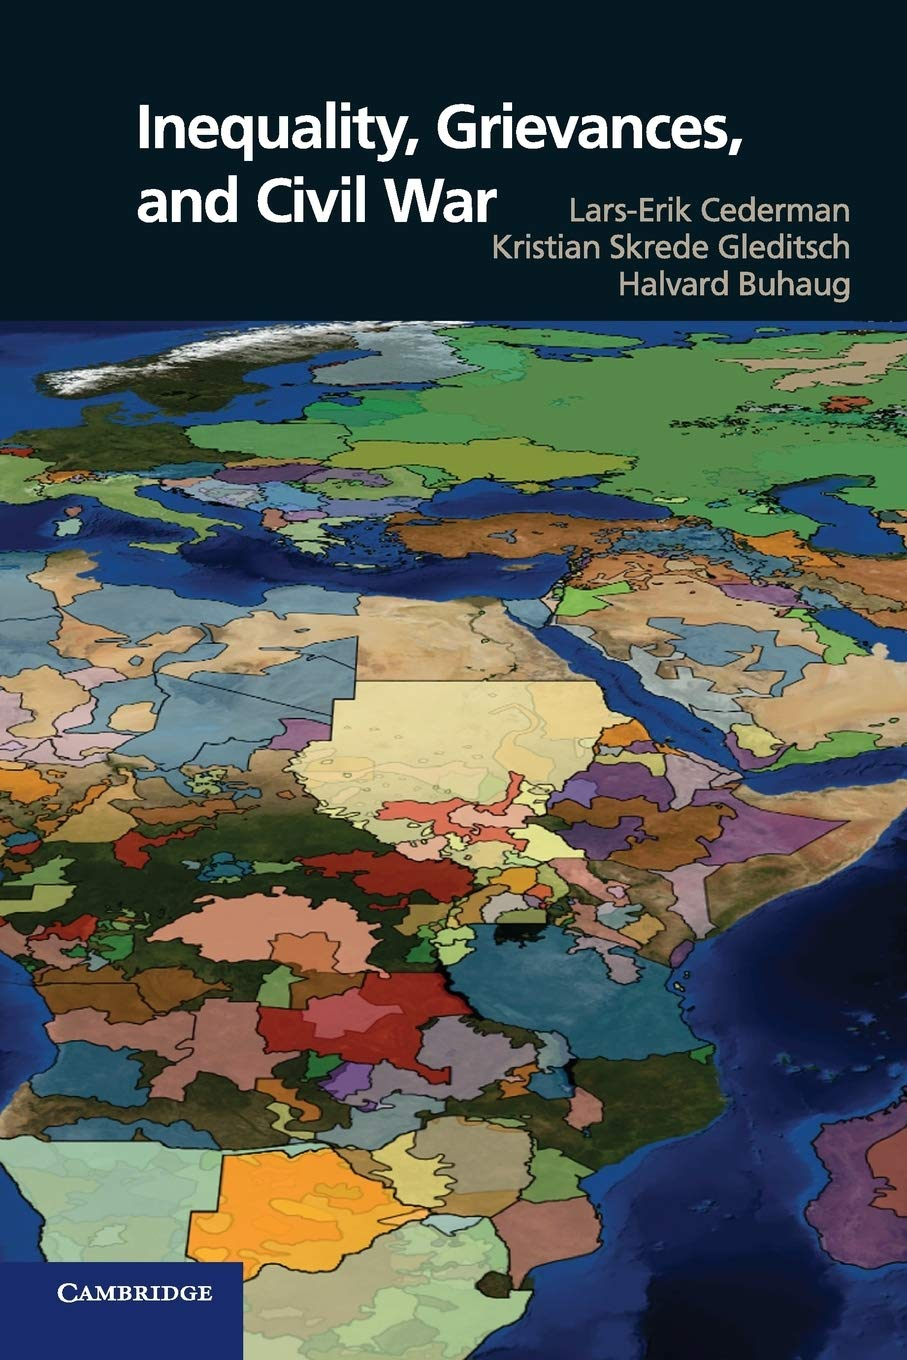
\includegraphics[width = 0.9\textwidth]{img/cgb}

{\small Cederman, Gleditsch, and Buhaug (2013)}
\end{minipage}

\end{frame}
% ----------------------------------------------------

% ----------------------------------------------------
\begin{frame}
\frametitle{From horizontal inequalities to conflict}
\centering

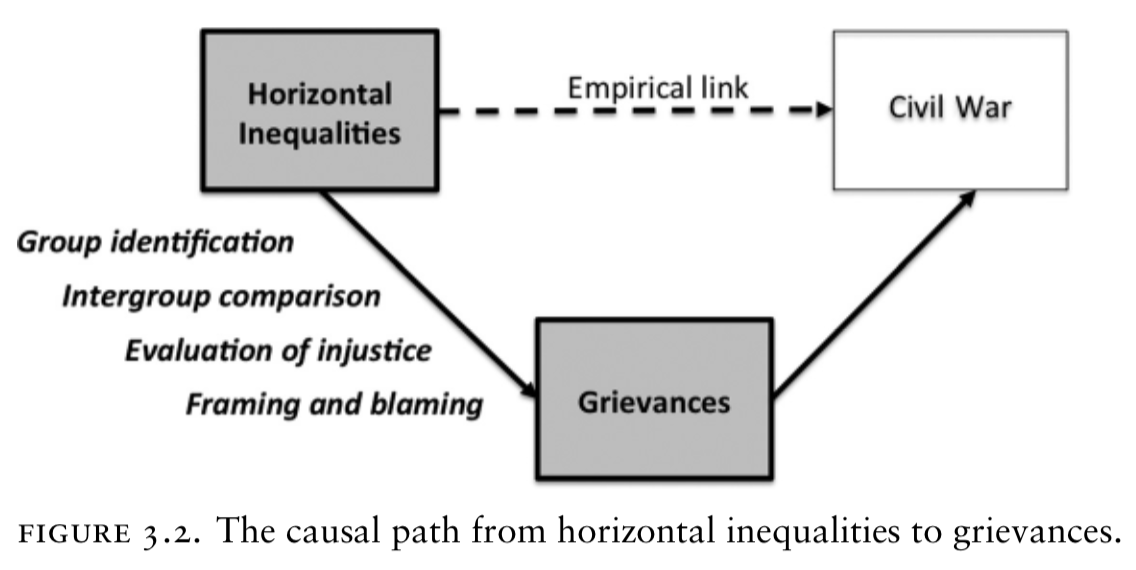
\includegraphics[width = 0.85\textwidth]{img/cgb_causal1}

\vspace{15pt}

{\small \textit{Source:} Cederman, Gleditsch, and Buhaug (2013)}

\end{frame}
% ----------------------------------------------------

% ----------------------------------------------------
\begin{frame}
\frametitle{From horizontal inequalities to conflict}
\centering

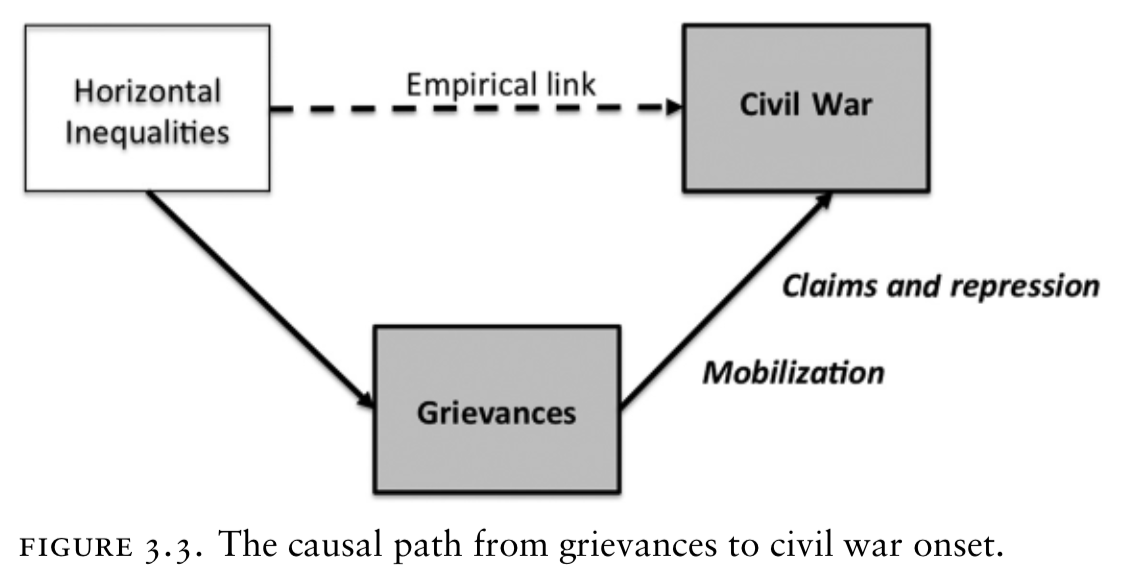
\includegraphics[width = 0.85\textwidth]{img/cgb_causal2}

\vspace{15pt}

{\small \textit{Source:} Cederman, Gleditsch, and Buhaug (2013)}

\end{frame}
% ----------------------------------------------------

% ----------------------------------------------------
\begin{frame}
\frametitle{Measuring grievances}
\centering

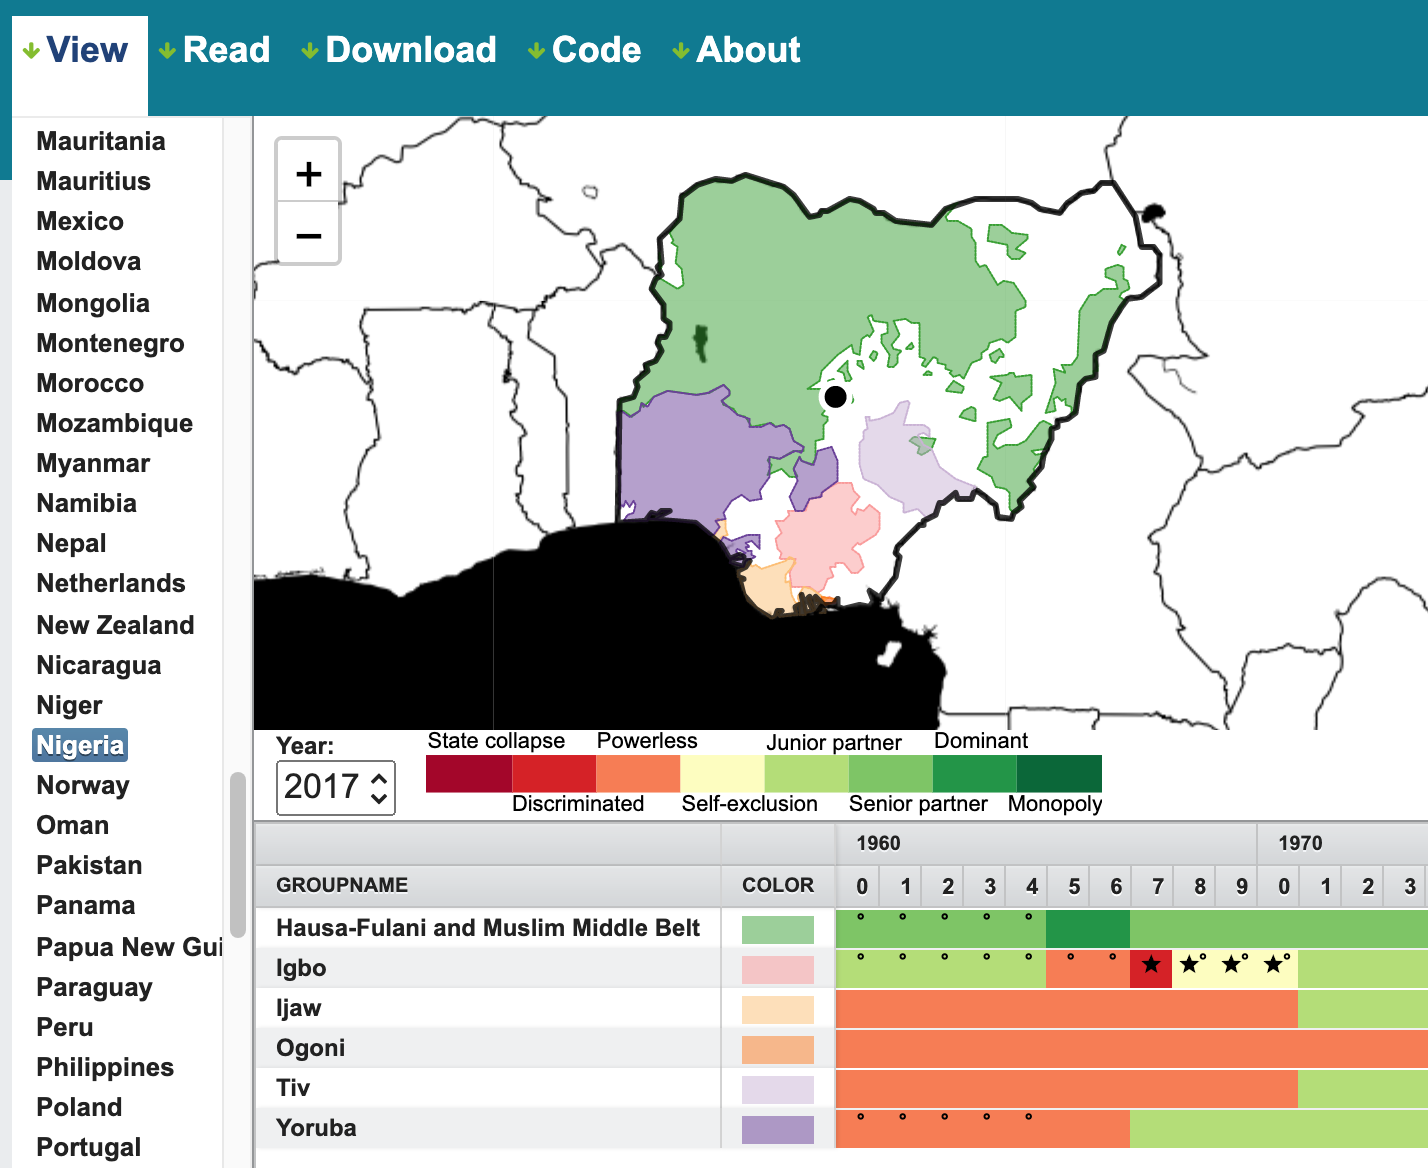
\includegraphics[width = 0.8\textwidth]{img/epr_nigeria}

\vspace{10pt}

{\small Ethnic Power Relations dataset (\url{https://growup.ethz.ch/})}

\end{frame}
% ----------------------------------------------------

% ----------------------------------------------------
\begin{frame}
\frametitle{Testing the effect of grievances}
\centering

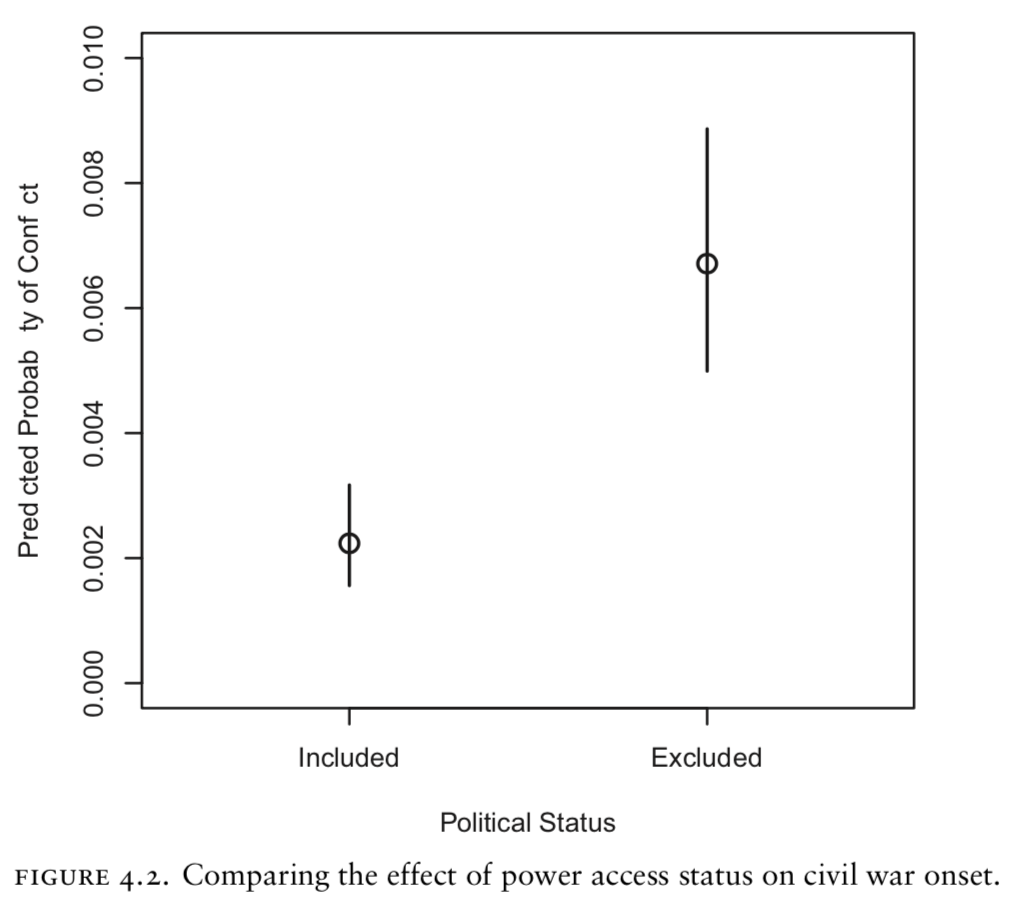
\includegraphics[width = 0.5\textwidth]{img/cgb_effect_exclusion}

\vspace{10pt}

{\small \textit{Source:} Cederman, Gleditsch, and Buhaug (2013)}

\vspace{15pt}

\begin{itemize}
  \item Being excluded from government linked to increased probability of conflict
\end{itemize}

\end{frame}
% ----------------------------------------------------

% ----------------------------------------------------
\begin{frame}
\frametitle{Testing the effect of grievances}
\centering

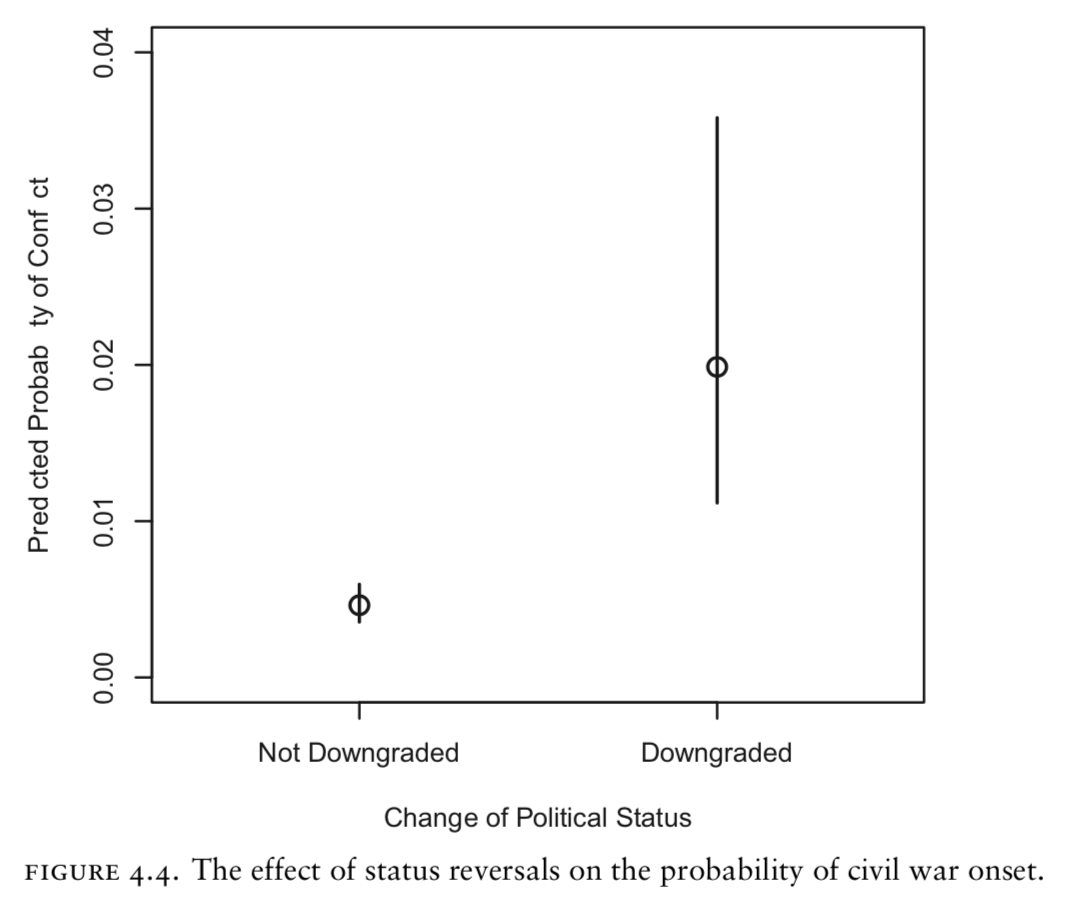
\includegraphics[width = 0.5\textwidth]{img/cgb_effect_downgrading}

\vspace{10pt}

{\small \textit{Source:} Cederman, Gleditsch, and Buhaug (2013)}

\vspace{15pt}

\begin{itemize}
  \item Losing status linked to increased probability of conflict
\end{itemize}

\end{frame}
% ----------------------------------------------------

% ----------------------------------------------------
\begin{frame}
\frametitle{The Cold War effect}
\centering

\begin{itemize}
  \item What about the effect of the \textit{international system} on domestic conflict?
  \item<2-> Another take: How global factors affected the \textit{technology of rebellion}
  \begin{itemize}
    \item[] {\footnotesize Balcells \& Kalyvas (\textit{American Political Science Review}, 2010)}
  \end{itemize}
  \item<3-> Remember the types:
  \begin{itemize}
    \item Irregular conflicts (guerrilla groups against conventional armies)
    \item Conventional civil wars (all conventional armies, clear frontlines)
    \item Symmetric non-conventional
  \end{itemize}
  \item<3-> Q: Did the change in the international system (end of Cold War) affect the way civil wars are fought?
\end{itemize}

\end{frame}
% ----------------------------------------------------

% ----------------------------------------------------
\begin{frame}
\frametitle{The Cold War effect (during \& after)}
\centering

\begin{itemize}
  \item Main idea: superpower support in `proxy wars' increased insurgents' capacity, that's why we see so many irregular wars
  \item How? Material support, ideological support, training...
  \item Support to both sides
  \begin{itemize}
    \item E.g. the USSR supported the government of Mozambique and US supported RENAMO
  \end{itemize}
  \item<2-> After the Cold War, USSR support disappears and US no longer has incentives, and previously existing states collapse and armies fragment
  \item<2-> Consequence? Increase in conventional and SNC wars
\end{itemize}

\end{frame}
% ----------------------------------------------------


% ----------------------------------------------------
\begin{frame}
\frametitle{The Cold War effect (during \& after)}
\centering

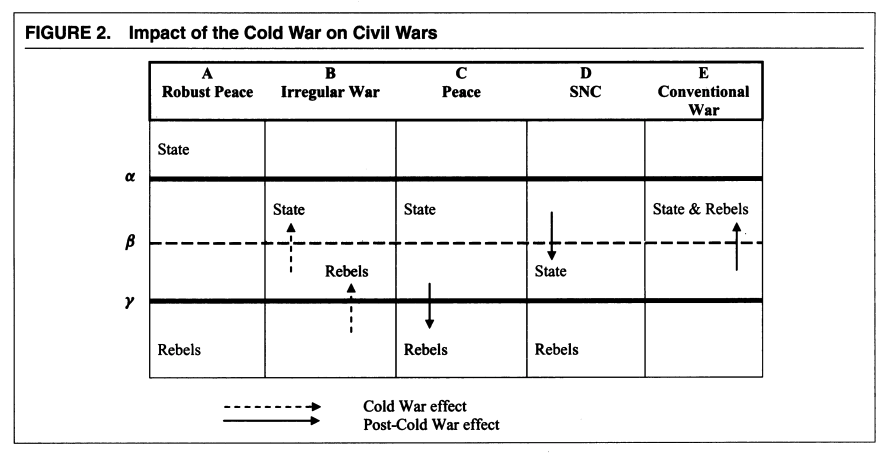
\includegraphics[width = 0.9\textwidth]{img/kalyvas_balcells_cold_war}

\begin{itemize}
  \item Above $\alpha$: state is too strong (stable peace)
  \item Above $\beta$: able to use conventional armies
  \item Above $\gamma$: able to use irregular warfare
  \item Below $\gamma$: not enough military capacity (bandits, terrorists, etc)
\end{itemize}

\end{frame}
% ----------------------------------------------------

% ----------------------------------------------------
\begin{frame}
\frametitle{The golden age of the \BGyellow{guerrillas}}
\centering

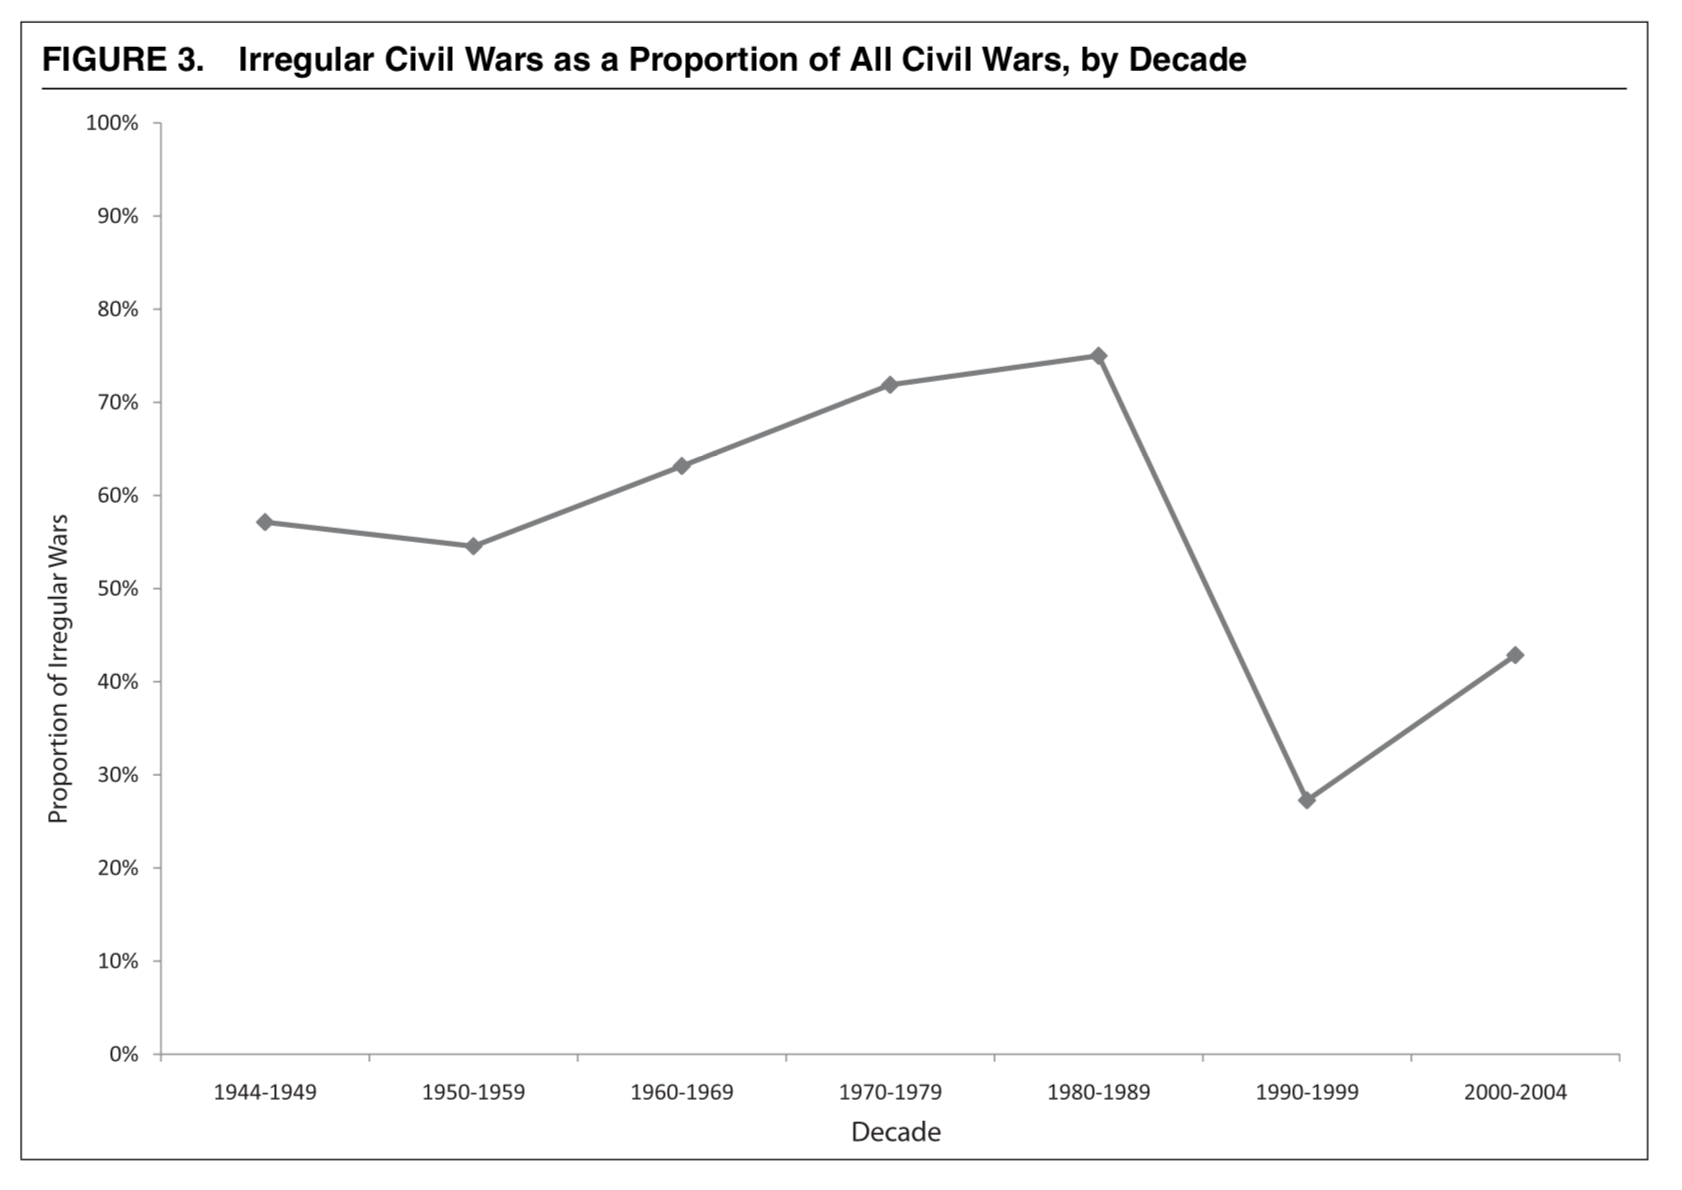
\includegraphics[width = \textwidth]{img/kalyvas_balcells_irr}

\end{frame}
% ----------------------------------------------------

% ----------------------------------------------------
\begin{frame}
\frametitle{The golden age of the \BGyellow{guerrillas}}
\centering

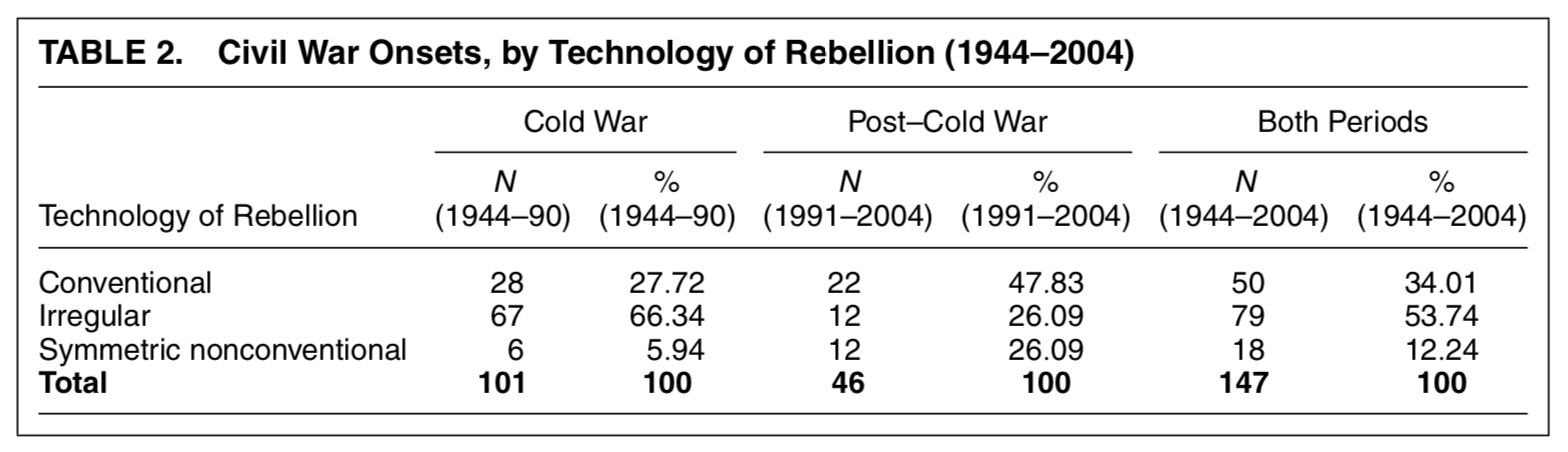
\includegraphics[width = \textwidth]{img/kalyvas_balcells_table}

\end{frame}
% ----------------------------------------------------

% ----------------------------------------------------
\begin{frame}
\frametitle{Wrapping up: explaining why civil wars break out}
\centering

\begin{itemize}
  \item<1-> Two key perspectives in academic research and policy-making
  \item<2-> \BGyellow{Greed / opportunity}
    \begin{itemize}
      \item How \textbf{viable} is to launch in insurgency?
      \item Economic and rational analysis of war onset
      \item Dismissing motivational factors (ethnicity, discrimination, etc)
    \end{itemize}
  \item<3-> \BGyellow{Grievance / motivation}
  \begin{itemize}
    \item Effect of \textbf{horizontal inequalities} on conflict
    \item Affects decision to fight, recruitment, internal cohesion...
    \item Critique to greed studies: need to measure this properly
  \end{itemize}
\end{itemize}

\end{frame}
% ----------------------------------------------------

% ----------------------------------------------------
\begin{frame}
\frametitle{Beyond greed vs grievance}
\centering

\begin{itemize}
  \item \textbf{No unique perspective is sufficient} to explain civil wars \textit{on its own}
  \item Recent research (and policy) focuses on combining them, e.g:
  \begin{itemize}
    \item<2-> Grievances can complement resource-based models of collective action (no extraction without representation)
    \item<3-> State capacity is probably the most important factor, but also includes a cultural aspect (nation-building)
    \item<4-> Opportunistic or \textit{greedy} leaders can co-exist with ideology-motivated participants
  \end{itemize}
  \item<5-> Alternative points of view: e.g., the role of the international system vs explanations that only focus on \textit{domestic} factors
\end{itemize}

\end{frame}
% ----------------------------------------------------

% ----------------------------------------------------
\begin{frame}
\frametitle{Beyond conflict onset}
\centering

\begin{itemize}
  \item Main focus is on civil war onset, which roughly tries to explain why at some point individuals decide to use organized violence against the state
  \item But if we care about civil wars because of the human suffering (or even economic consequences), we should look at least at two different things
  \begin{itemize}
    \item \BGyellow{How long do wars last?}
    \item \BGyellow{Why do wars break out again?} (we'll see this in the postwar week)
  \end{itemize}
\end{itemize}

\end{frame}
% ----------------------------------------------------



% ----------------------------------------------------
\begin{frame}
\frametitle{How \BGyellow{long} do civil wars last?}
\centering

\begin{itemize}
  \item Fearon (2004) `Why do some civil wars last so much longer than others?'
  \item Two types of particularly long conflicts:
  \begin{itemize}
    \item Conflicts where rebel groups receive funding from contraband activities: diamonds, coca, opium...
    \item `Sons-of-the-soil' conflicts: ethnic minority in the periphery against a dominant ethnic group that supports migrants into the periphery
  \end{itemize}
  \item<2-> Commitment problems
  \begin{itemize}
    \item Why would I stop fighting and reach a negotiated settlement?
    \item Wartime contraband is making me rich even if fighting is costly
    \item I'm sending migrants of my group to your region, which will increase in local power in the future
  \end{itemize}
\end{itemize}
% Balcells, L., & Kalyvas, S. N. (2014). Does Warfare Matter? Severity, Duration, and Outcomes of Civil Wars. Journal of Conflict Resolution, 58(8), 1390–1418.

\end{frame}
% ----------------------------------------------------

% ----------------------------------------------------
\begin{frame}
\frametitle{How \BGyellow{long} do civil wars last?}
\centering

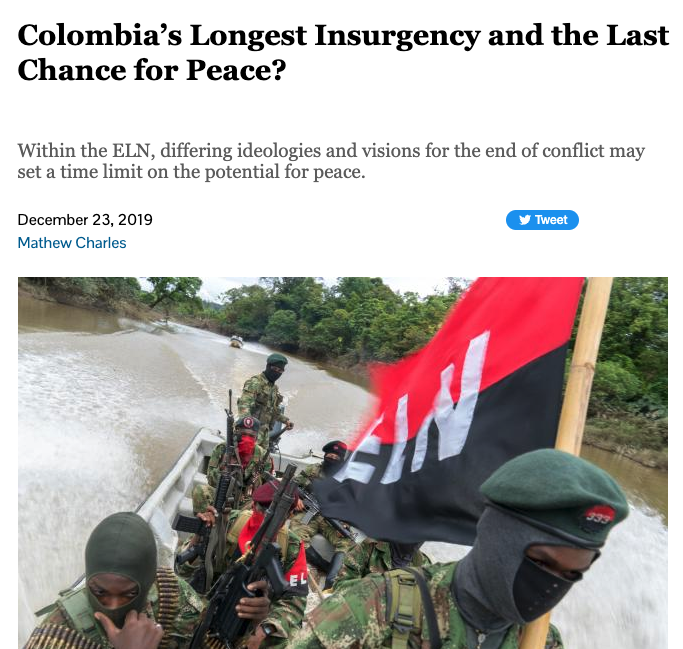
\includegraphics[width = \textwidth]{img/colombia_duration}

\end{frame}
% ----------------------------------------------------

% ----------------------------------------------------
\begin{frame}
\frametitle{How \BGyellow{long} do civil wars last?}
\centering

\begin{itemize}
  \item But another explanation is that the way a civil war is fought could also impact its duration
  \item Why did civil wars in Colombia, Guatemala, ... last for so long?
  \begin{itemize}
    \item not the same, but why did the Troubles in NI or ETA in Spain last for so long?
  \end{itemize}
  \item Ideas?
\end{itemize}

\end{frame}
% ----------------------------------------------------

% ----------------------------------------------------
\begin{frame}
\frametitle{How \BGyellow{long} do civil wars last?}
\centering

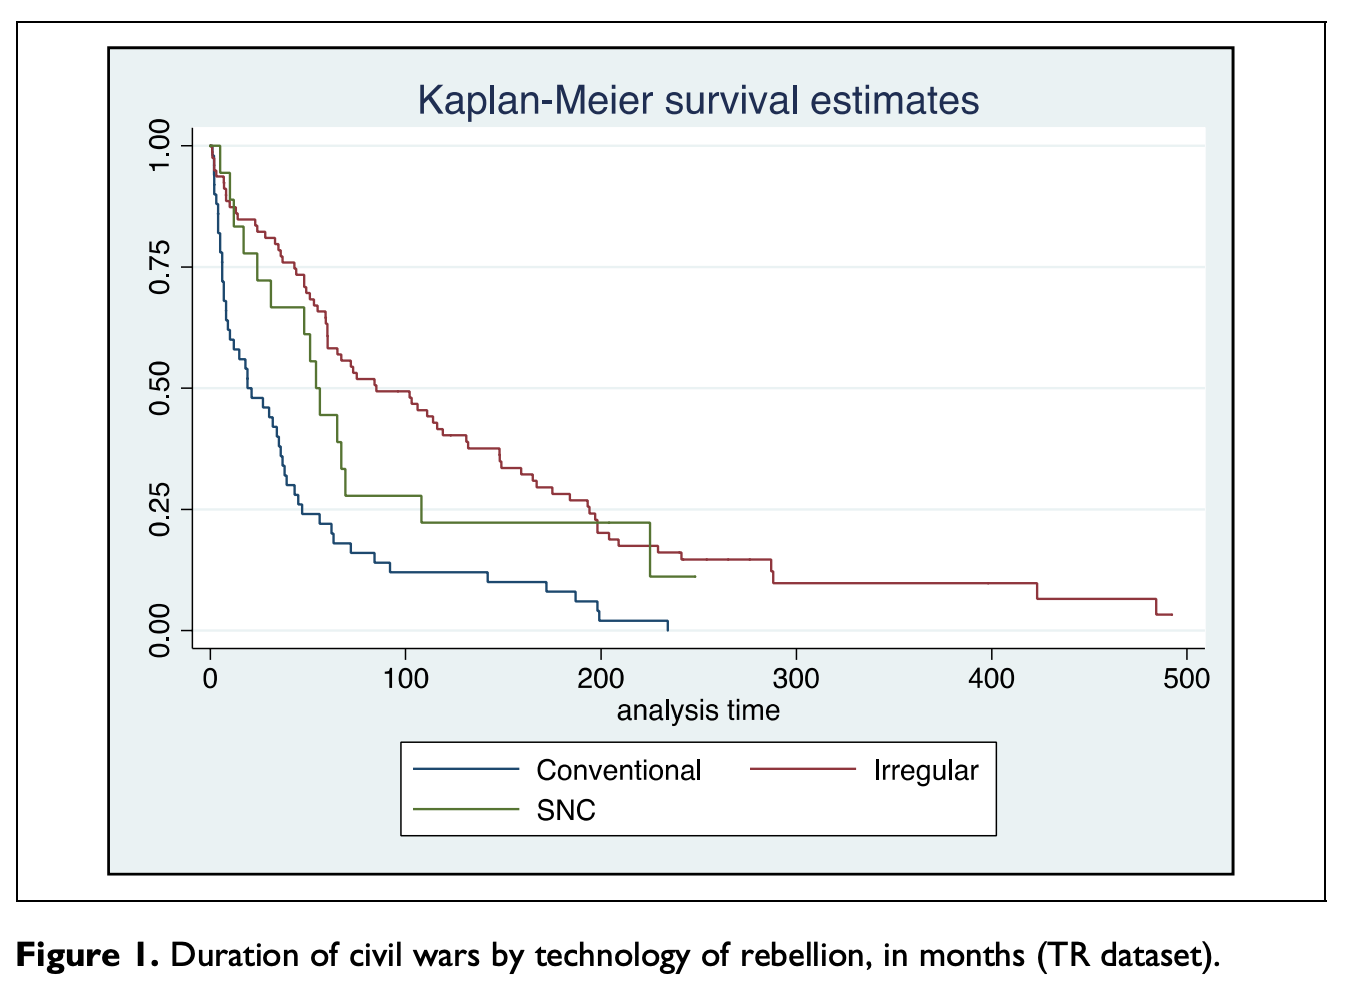
\includegraphics[width = 0.8\textwidth]{img/balcells_kalyvas_duration}

% \vspace{10pt}

\begin{itemize}
  \item Balcells \& Kalyvas (\textit{Journal of Conflict Resolution,} 2014)
  \item Looking at the duration depending on \textbf{technology of rebellion}
\end{itemize}

% Balcells, L., & Kalyvas, S. N. (2014). Does Warfare Matter? Severity, Duration, and Outcomes of Civil Wars. Journal of Conflict Resolution, 58(8), 1390–1418.

\end{frame}
% ----------------------------------------------------


% ----------------------------------------------------
\begin{frame}
\frametitle{How \BGyellow{long} do civil wars last?}
\centering

\begin{itemize}
  \item What about \textbf{grievances}?
  \item How can they impact the duration of wars?
  \item And can they explain why some conflicts are so durable?
\end{itemize}

\end{frame}
% ----------------------------------------------------

% ----------------------------------------------------
\begin{frame}
\frametitle{Next seminar}
\centering

\begin{minipage}{0.55\textwidth}\centering
\begin{itemize}
  \item Anand Gopal, `The other Afghan women' (\textit{New Yorker,} Sept 2021)
  \item Why women turned against the US and supported the Taliban
\end{itemize}
\end{minipage}\hfill
\begin{minipage}{0.44\textwidth}\centering
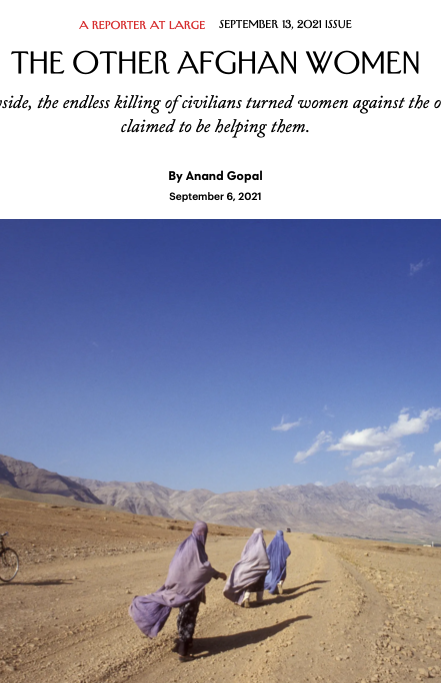
\includegraphics[width = \textwidth]{img/gopal}
\end{minipage}

\end{frame}
% ----------------------------------------------------

\end{document}
